% !TeX spellcheck = en_US
\chapter{Methodology}%

\section{Introduction}%

The proposed method aims to provide a framework for optimizing various parameters of an industrial robot. By effectively utilizing the redundant degrees of freedom mentioned in Chapter \ref{OBJECTIVE}, this method is applicable to robotic milling operations and WAAM processes. The successful implementation of this methodology improves the robot's overall performance and efficiency, leading to increased productivity in industrial operations.

The first step involves constructing a basic model that captures the kinematics and dynamics of an industrial robot. To test the method in a simple case, the first tests are performed on a non-redundant 6-DoF model. After validation on this simple model, redundant degrees of freedom are introduced. After that, the method is connected to CAM software to be tested in more complex scenarios.

Once the basic mathematical model is established, various optimization algorithms are implemented to determine the optimal values for each parameter associated with the redundant degrees of freedom. These methods and optimization algorithms will consider the industrial robot's specific objectives and constraints, like energy consumption, feed rates, and accelerations. The validation process entails conducting real-world tests and simulations to evaluate optimized parameter performance and verify the effectiveness of our proposed methodology.


\section{General Methodology for Process Analysis}
\subsection{General Methodology}\label{general}

The flowchart in figure \ref{BasicScore} shows the interdependence of a tool path, the used manufacturing machine, the material, and set boundary conditions. The machine defines general parameters like reach, DoF, maximum feed rates, and manufacturing process (additive or subtractive). It can be a 6-axis CNC machine or an 8-DoF industrial robot. The part is referred to as the finished geometry as designed in CAD. The material is a user-defined element from which the part should be manufactured. The elements "Machine", "Part" and "Material" directly influence the toolpath that is necessary for manufacturing. The machine, for example, defines if the spindle or the work piece itself needs to be tilted to achieve the desired geometric features. The material and available end-mills are also influencing the depth of cut and required passes to achieve the desired geometries. 

\begin{figure}[H]
	\centerline{\includegraphics[scale=.65]{figures/BasicScore.png}}
	\caption{Interdependence of various parameters}
	\label{BasicScore}
\end{figure}

As the tool path is only a relative movement in regards to the work piece, the user is required to define further parameters before starting the manufacturing process. One example is the positioning of the raw stock material in the machine itself and defining the coordinate system that is used as a reference for the tool center point (TCP). These two boundary conditions have to be in accordance with the  machine's capabilities and can require extensive knowledge about the machine as well as performed process.

One of the other parameters that needs to be defined is the positioning or constraining of redundant DoF. One of the simplest cases to illustrate this constraining, is when using a 6-DoF robot for milling operations. In milling, the TCP position is defined by three coordinates, namely X, Y, and Z, as well as the rotation around the X and Y axes. The rotation around the Z-axis needs to be defined manually, as the spindle has rotatory symmetry around that axis. This constraint ensures that the robot maintains a specified pose while performing milling operations. The rotation around the Z axis can be set to any arbitrarily set value but can influence the overall process parameters significantly. 

After the constraints are set and the tool path is generated, various process parameters can be analyzed. Some of the more prominent parameters are the total angular travel of a specific joint or the total angular acceleration. In addition to these numerical values, the user can define a specific importance for the analyzed process parameters and, with a weighting of all available process parameters, calculate an overall score of the determined tool path.


%More information regarding the parameters and weights is presented in chapter \ref{pp}.

\subsection{Process Parameters}\label{pp}


Table \ref{procesparameters} presents a comprehensive overview of the various process parameters that can be derived from a tool path executed by an industrial robot. One of the key parameters is the joint position, which is typically recorded as an array containing the rotational or extension values of each rotary or linear joint at every time-step. This information serves as a basis for determining subsequent parameters such as velocity, acceleration, and jerk. By employing a forward kinematics approach, it becomes possible to determine the position (X Y Z position) and orientation (rotation) of the TCP (Tool Center Point). Additionally, the acceleration and jerk can be calculated by taking the respective derivatives with respect to time. These derived parameters, along with the joint positions, are all stored in the form of arrays that capture the temporal changes in their respective values.


Another crucial factor in industrial robot tool path execution is the stiffness value. This value specifically refers to the stiffness in the direction of the highest contact forces, or the most critical direction. In certain machining scenarios, such as when cutting a slot with full engagement, the stiffness in the cutting direction may be of lesser importance compared to the stiffness in the perpendicular direction of the cut.

Maintaining high stiffness in the orthogonal cutting direction is vital, as it helps minimize deviations from the desired mid-axis of the slot. Conversely, when high contact forces are combined with low stiffness, it can result in significant deviations in the final dimensions of the machined part.
To determine the stiffness value, a finite-element analysis, multi-body simulation or CAM simulation can be employed. These simulations provide the necessary data, which is also stored in the form of an array, to extract the stiffness values for analysis and optimization purposes.


Estimating the energy usage in industrial robot applications is another crucial aspect that can be achieved through multi-body simulations. To accurately estimate energy consumption, it is essential to have a correct 3D model that includes information about the weight and its distribution of the workpiece, as well as the robot joints.

One significant factor to consider is the change in weight of the workpiece. In additive manufacturing processes, the weight of the workpiece typically increases due to material deposition, while in subtractive manufacturing processes, such as milling, the weight decreases as material is removed.

Furthermore, in cases where the industrial robot is utilized for milling operations, it becomes necessary to estimate the cutting forces generated during the process. This helps in evaluating the energy requirements for milling. On the other hand, if the robot is employed for WAAM, the power usage can be extracted from the G-code by analyzing the duration for which the welding torch remains active. This information allows for the determination of the power consumption associated with the welding process. The energy usage is measured in Watts and, similar to the other parameters mentioned earlier, is also represented in the form of an array to capture the variations in energy consumption over time.

In order to prolong the lifespan of an industrial robot, it is crucial to consider the load on individual joints. One important indicator of joint load is the number of direction changes that a joint undergoes during its operation. High-frequency rotation changes can result in significant degradation and loss of precision during manufacturing processes.
This process parameter, known as the number of direction changes, is a scalar value that can be derived from the angular position of each joint. By analyzing the joint position data, the total travel of a joint can be determined by taking the integral of the joint position over time.

Programs or tool paths that require less joint travel are generally more desirable as they reduce the time spent on non-value-adding work. By minimizing the number of direction changes and optimizing the joint travel, the stress and wear on the robot joints can be reduced, thereby extending the overall lifespan of the robot system.

Total energy usage is a key parameter that can be measured directly during the manufacturing process. It provides valuable insights into the overall energy consumption of the industrial robot system. This parameter can be obtained by monitoring the energy usage in real-time or by integrating the time-series data of the energy consumption.

To measure the energy usage during the manufacturing process, various techniques and technologies can be employed. These may include energy meters or sensors that directly measure the power consumption of the robot system. By continuously monitoring the energy usage, it becomes possible to accurately determine the total energy consumed throughout the manufacturing process.

Alternatively, if direct measurement of energy usage is not available, the energy consumption can be estimated by integrating the time-series data of the energy consumption. This involves summing up the energy consumed at each time-step over the duration of the manufacturing process. Although this estimation method may not be as accurate as direct measurement, it can still provide valuable insights into the overall energy usage.

By analyzing the total energy usage, manufacturers can identify energy-intensive processes or operations, optimize energy consumption, and implement strategies to reduce overall energy consumption, leading to cost savings and environmental benefits.

The singularity analysis parameter can be represented either as a time-series or as a single numerical value. It is based on the smallest eigenvalue of the Jacobian matrix, which is calculated using the robot's current configuration. This parameter can be stored in array form, capturing the changes in singularity analysis over time. Alternatively, only the smallest eigenvalue encountered during the entire tool path can be recorded.

The analysis of the singularity time-series can be used to optimize non-optimal poses, ensuring that the robot avoids singular configurations that may lead to reduced performance or unexpected behavior. It can also serve as an indicator to detect and monitor if a singularity is reached during the operation.

Another important parameter is the cycle time, which represents the time required to execute the G-code. Various factors can influence the cycle time, such as feed rates, engagement depth of a cutting tool, or wire feed rates in the case of additive manufacturing processes. By adjusting these parameters, manufacturers can significantly reduce or increase the cycle time, optimizing the efficiency and productivity of the manufacturing process.

Analyzing and optimizing the cycle time helps to streamline operations, reduce production time, and enhance overall productivity. It allows manufacturers to identify opportunities for improvement and make informed decisions regarding process parameters, leading to increased throughput and cost savings.


The reachability index and the collision index are binary parameters used to determine the feasibility of executing a program in an industrial robot system.

The reachability index indicates whether all the necessary points defined in the tool path are inside the working volume of the robot and can be reached by the robot's TCP. This parameter helps ensure that the robot can physically access all the required positions in the work area. If any point is found to be outside the reachable workspace, it may indicate a need for adjustments in the program or the robot's positioning capabilities.

The collision index is used to determine if any potential collisions could occur between any part of the robot or the end-effector and the workpieces or other objects in the environment. This parameter is particularly important in scenarios involving WAAM systems, where loose wires can change their position depending on the robot's pose. It helps to prevent potential collisions that could lead to damage to the workpiece, the robot, or other equipment.

To ensure safe and efficient operations, both the reachability index and the collision index are evaluated before the G-code program is executed. If all positions in the tool path are reachable and no collision is expected, the G-code is considered safe for production and can be executed. If any issues are identified, adjustments can be made to the program or the robot's configuration to ensure proper reachability and collision avoidance.


\begin{table}[H]
	\centering
	\begin{tabular}{||l|r||}
		Process Parameter & Numerical Form\\
		\hline
		\hline
		\hline
		
		Angular position of each joint & Time series\\
		Angular velocity of each joint & Time series\\
		Angular acceleration of each joint& Time series\\
		Angular jerk of each joint& Time series\\
		\hline
		\hline	
		
		TCP coordinates X & Time series\\
		TCP coordinates Y & Time series\\
		TCP coordinates Z & Time series\\
		\hline
		\hline
		TCP acceleration in X & Time series\\
		TCP acceleration in Y & Time series\\
		TCP acceleration in Z & Time series\\
		\hline
		\hline
		Stiffness value & Time series\\
		
		
		Continuous energy usage & Time series\\
		\hline
		\hline
		Direction changes of each joint& Scalar value\\
		Total travel of each joint& Scalar value\\
		Total energy usage & Scalar value\\
		Singularity Analysis & Scalar value\\
		Cycle time & Scalar value\\
		\hline
		\hline
		Reachability index & Binary value\\
		Collision index & Binary value\\
		\hline
		\hline
		
	\end{tabular}
	
	
	\caption{Process parameter and their numerical form}
	\label{procesparameters}
\end{table}

Figure \ref{ParamsFlow} visualizes how the different parameters are interconnected. It is clearly visible that all parameters except cycle time can be derived from the angular position of the joints. This is a clear indicator of the importance of that information. The angular position data provides essential information for analyzing and optimizing the performance, efficiency, and safety of the robot system. By monitoring and analyzing the joint positions, manufacturers can gain insights into various aspects of the robot's operation and make informed decisions to optimize productivity.

\begin{figure}[H]
	\centerline{\includegraphics[scale=.55]{figures/Flow.png}}
	\caption{Parameter Flowchart}
	\label{ParamsFlow}
\end{figure}


\subsection{User-Defined Weights}\label{weights}
To assess if a tool path is optimal or offers the possibility for improvement, a score or rating value is required that takes the process parameters and their importance into account. 

Determining the relative importance of different parameters can involve subjective judgments, expert knowledge, and consideration of specific manufacturing constraints. For example, in some cases, minimizing cycle time may be the primary objective, while in others, energy usage may take precedence.

To quantify the optimality of a tool path, manufacturers may assign weights or importance factors to each parameter based on their specific requirements. These weights can reflect the relative significance of each parameter in achieving the desired manufacturing outcomes. A weighted sum or scoring method can then be used to evaluate and compare different tool paths based on the aggregated scores of the individual parameters.

It's important to note that the subjective weighing of parameters can vary between different manufacturing scenarios and may require continuous evaluation and adjustment based on changing priorities or goals.

The score of a tool path is then calculated as shown in table \ref{weighting}. Each process parameter can take a value in the range 0-100. 0 being the least optimal, while 100 represents the optimal.

\begin{table}[H]
	\centering
	\begin{tabular}{||l|r|r|r||}
		Process Parameters & Local rating & Importance & Local score\\
		\hline
		\hline
		\hline
		
		Process Parameter 1 & 74 & 0.5 & 37\\
		Process Parameter 2 & 34& 0.1&3.4\\
		Process Parameter 3& 65& 0.1&6.5\\
		Process Parameter 4& 22&0.3&6.6\\
		\hline
		\hline
		\hline
		Global Score& & &53,5\\
		\hline
		\hline
	\end{tabular}
	
	\caption{Calculation of a tool path score}
	\label{weighting}
\end{table}

Calculating a local rating is not a straight-forward approach. The first problem is that based on a singular value like "direction changes," it is not possible to determine a local rating as it is not clear if that value is close to optimal or far from it.
The solution to this problem is calculating the tool path with different boundary conditions like workplace placement or constraints like rotation around the C-axis.
Figure \ref{Localscore} shows how a local score can be calculated by means of variation. Each variation leads to a different number of direction changes in joint 1. The local score is calculated by essentially applying a Min-Max scaler.

\begin{figure}[H]
	\centerline{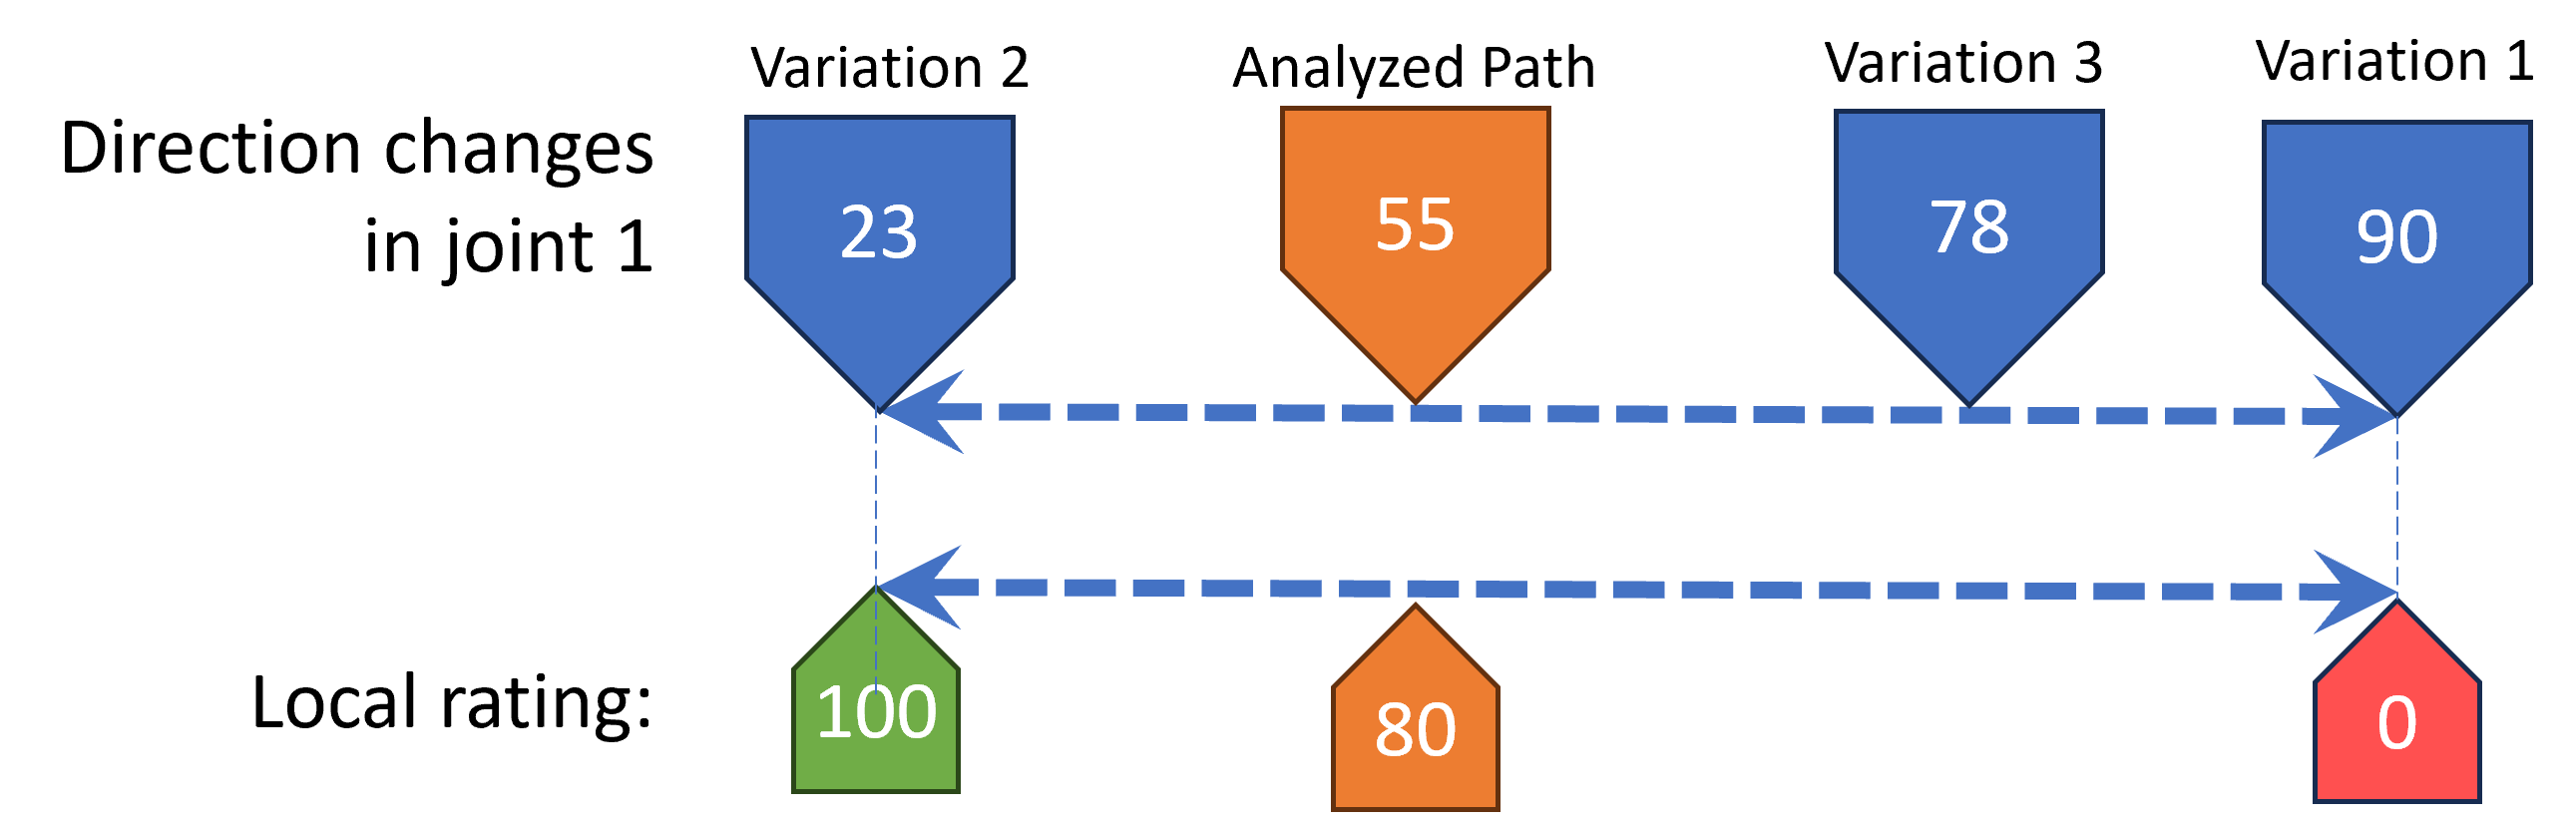
\includegraphics[scale=.65]{figures/localscore.png}}
	\caption{Calculation of the local score trough variation}
	\label{Localscore}
\end{figure}

The second problem is connected to the time-series format of the recorded parameters. To acquire a local score, the time series need to be transformed into a scalar value.


Each time series requires individual analysis


What time series is even necessary ? 


What parameters form a time series needs to be extracted ?





